\documentclass[1p]{elsarticle_modified}
%\bibliographystyle{elsarticle-num}

%\usepackage[colorlinks]{hyperref}
%\usepackage{abbrmath_seonhwa} %\Abb, \Ascr, \Acal ,\Abf, \Afrak
\usepackage{amsfonts}
\usepackage{amssymb}
\usepackage{amsmath}
\usepackage{amsthm}
\usepackage{scalefnt}
\usepackage{amsbsy}
\usepackage{kotex}
\usepackage{caption}
\usepackage{subfig}
\usepackage{color}
\usepackage{graphicx}
\usepackage{xcolor} %% white, black, red, green, blue, cyan, magenta, yellow
\usepackage{float}
\usepackage{setspace}
\usepackage{hyperref}

\usepackage{tikz}
\usetikzlibrary{arrows}

\usepackage{multirow}
\usepackage{array} % fixed length table
\usepackage{hhline}

%%%%%%%%%%%%%%%%%%%%%
\makeatletter
\renewcommand*\env@matrix[1][\arraystretch]{%
	\edef\arraystretch{#1}%
	\hskip -\arraycolsep
	\let\@ifnextchar\new@ifnextchar
	\array{*\c@MaxMatrixCols c}}
\makeatother %https://tex.stackexchange.com/questions/14071/how-can-i-increase-the-line-spacing-in-a-matrix
%%%%%%%%%%%%%%%

\usepackage[normalem]{ulem}

\newcommand{\msout}[1]{\ifmmode\text{\sout{\ensuremath{#1}}}\else\sout{#1}\fi}
%SOURCE: \msout is \stkout macro in https://tex.stackexchange.com/questions/20609/strikeout-in-math-mode

\newcommand{\cancel}[1]{
	\ifmmode
	{\color{red}\msout{#1}}
	\else
	{\color{red}\sout{#1}}
	\fi
}

\newcommand{\add}[1]{
	{\color{blue}\uwave{#1}}
}

\newcommand{\replace}[2]{
	\ifmmode
	{\color{red}\msout{#1}}{\color{blue}\uwave{#2}}
	\else
	{\color{red}\sout{#1}}{\color{blue}\uwave{#2}}
	\fi
}

\newcommand{\Sol}{\mathcal{S}} %segment
\newcommand{\D}{D} %diagram
\newcommand{\A}{\mathcal{A}} %arc


%%%%%%%%%%%%%%%%%%%%%%%%%%%%%5 test

\def\sl{\operatorname{\textup{SL}}(2,\Cbb)}
\def\psl{\operatorname{\textup{PSL}}(2,\Cbb)}
\def\quan{\mkern 1mu \triangleright \mkern 1mu}

\theoremstyle{definition}
\newtheorem{thm}{Theorem}[section]
\newtheorem{prop}[thm]{Proposition}
\newtheorem{lem}[thm]{Lemma}
\newtheorem{ques}[thm]{Question}
\newtheorem{cor}[thm]{Corollary}
\newtheorem{defn}[thm]{Definition}
\newtheorem{exam}[thm]{Example}
\newtheorem{rmk}[thm]{Remark}
\newtheorem{alg}[thm]{Algorithm}

\newcommand{\I}{\sqrt{-1}}
\begin{document}

%\begin{frontmatter}
%
%\title{Boundary parabolic representations of knots up to 8 crossings}
%
%%% Group authors per affiliation:
%\author{Yunhi Cho} 
%\address{Department of Mathematics, University of Seoul, Seoul, Korea}
%\ead{yhcho@uos.ac.kr}
%
%
%\author{Seonhwa Kim} %\fnref{s_kim}}
%\address{Center for Geometry and Physics, Institute for Basic Science, Pohang, 37673, Korea}
%\ead{ryeona17@ibs.re.kr}
%
%\author{Hyuk Kim}
%\address{Department of Mathematical Sciences, Seoul National University, Seoul 08826, Korea}
%\ead{hyukkim@snu.ac.kr}
%
%\author{Seokbeom Yoon}
%\address{Department of Mathematical Sciences, Seoul National University, Seoul, 08826,  Korea}
%\ead{sbyoon15@snu.ac.kr}
%
%\begin{abstract}
%We find all boundary parabolic representation of knots up to 8 crossings.
%
%\end{abstract}
%\begin{keyword}
%    \MSC[2010] 57M25 
%\end{keyword}
%
%\end{frontmatter}

%\linenumbers
%\tableofcontents
%
\newcommand\colored[1]{\textcolor{white}{\rule[-0.35ex]{0.8em}{1.4ex}}\kern-0.8em\color{red} #1}%
%\newcommand\colored[1]{\textcolor{white}{ #1}\kern-2.17ex	\textcolor{white}{ #1}\kern-1.81ex	\textcolor{white}{ #1}\kern-2.15ex\color{red}#1	}

{\Large $\underline{12a_{1121}~(K12a_{1121})}$}

\setlength{\tabcolsep}{10pt}
\renewcommand{\arraystretch}{1.6}
\vspace{1cm}\begin{tabular}{m{100pt}>{\centering\arraybackslash}m{274pt}}
\multirow{5}{120pt}{
	\centering
	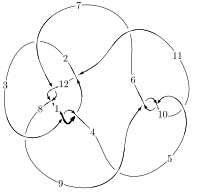
\includegraphics[width=112pt]{../../../GIT/diagram.site/Diagrams/png/1922_12a_1121.png}\\
\ \ \ A knot diagram\footnotemark}&
\allowdisplaybreaks
\textbf{Linearized knot diagam} \\
\cline{2-2}
 &
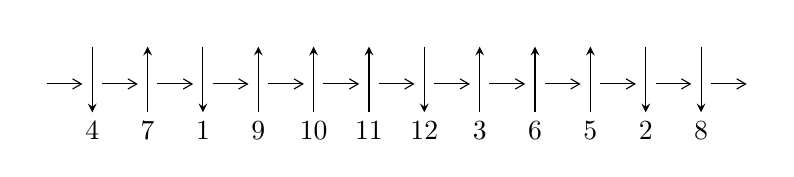
\begin{tikzpicture}[x=20pt, y=17pt]
	% nodes
	\node (C0) at (0, 0) {};
	\node (C1) at (1, 0) {};
	\node (C1U) at (1, +1) {};
	\node (C1D) at (1, -1) {4};

	\node (C2) at (2, 0) {};
	\node (C2U) at (2, +1) {};
	\node (C2D) at (2, -1) {7};

	\node (C3) at (3, 0) {};
	\node (C3U) at (3, +1) {};
	\node (C3D) at (3, -1) {1};

	\node (C4) at (4, 0) {};
	\node (C4U) at (4, +1) {};
	\node (C4D) at (4, -1) {9};

	\node (C5) at (5, 0) {};
	\node (C5U) at (5, +1) {};
	\node (C5D) at (5, -1) {10};

	\node (C6) at (6, 0) {};
	\node (C6U) at (6, +1) {};
	\node (C6D) at (6, -1) {11};

	\node (C7) at (7, 0) {};
	\node (C7U) at (7, +1) {};
	\node (C7D) at (7, -1) {12};

	\node (C8) at (8, 0) {};
	\node (C8U) at (8, +1) {};
	\node (C8D) at (8, -1) {3};

	\node (C9) at (9, 0) {};
	\node (C9U) at (9, +1) {};
	\node (C9D) at (9, -1) {6};

	\node (C10) at (10, 0) {};
	\node (C10U) at (10, +1) {};
	\node (C10D) at (10, -1) {5};

	\node (C11) at (11, 0) {};
	\node (C11U) at (11, +1) {};
	\node (C11D) at (11, -1) {2};

	\node (C12) at (12, 0) {};
	\node (C12U) at (12, +1) {};
	\node (C12D) at (12, -1) {8};
	\node (C13) at (13, 0) {};

	% arrows
	\draw[->,>={angle 60}]
	(C0) edge (C1) (C1) edge (C2) (C2) edge (C3) (C3) edge (C4) (C4) edge (C5) (C5) edge (C6) (C6) edge (C7) (C7) edge (C8) (C8) edge (C9) (C9) edge (C10) (C10) edge (C11) (C11) edge (C12) (C12) edge (C13) ;	\draw[->,>=stealth]
	(C1U) edge (C1D) (C2D) edge (C2U) (C3U) edge (C3D) (C4D) edge (C4U) (C5D) edge (C5U) (C6D) edge (C6U) (C7U) edge (C7D) (C8D) edge (C8U) (C9D) edge (C9U) (C10D) edge (C10U) (C11U) edge (C11D) (C12U) edge (C12D) ;
	\end{tikzpicture} \\
\hhline{~~} \\& 
\textbf{Solving Sequence} \\ \cline{2-2} 
 &
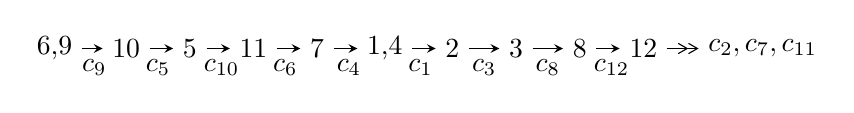
\begin{tikzpicture}[x=23pt, y=7pt]
	% node
	\node (A0) at (-1/8, 0) {6,9};
	\node (A1) at (1, 0) {10};
	\node (A2) at (2, 0) {5};
	\node (A3) at (3, 0) {11};
	\node (A4) at (4, 0) {7};
	\node (A5) at (81/16, 0) {1,4};
	\node (A6) at (49/8, 0) {2};
	\node (A7) at (57/8, 0) {3};
	\node (A8) at (65/8, 0) {8};
	\node (A9) at (73/8, 0) {12};
	\node (C1) at (1/2, -1) {$c_{9}$};
	\node (C2) at (3/2, -1) {$c_{5}$};
	\node (C3) at (5/2, -1) {$c_{10}$};
	\node (C4) at (7/2, -1) {$c_{6}$};
	\node (C5) at (9/2, -1) {$c_{4}$};
	\node (C6) at (45/8, -1) {$c_{1}$};
	\node (C7) at (53/8, -1) {$c_{3}$};
	\node (C8) at (61/8, -1) {$c_{8}$};
	\node (C9) at (69/8, -1) {$c_{12}$};
	\node (A10) at (11, 0) {$c_{2},c_{7},c_{11}$};

	% edge
	\draw[->,>=stealth]	
	(A0) edge (A1) (A1) edge (A2) (A2) edge (A3) (A3) edge (A4) (A4) edge (A5) (A5) edge (A6) (A6) edge (A7) (A7) edge (A8) (A8) edge (A9) ;
	\draw[->>,>={angle 60}]	
	(A9) edge (A10);
\end{tikzpicture} \\ 

\end{tabular} \\

\footnotetext{
The image of knot diagram is generated by the software ``\textbf{Draw programme}" developed by Andrew Bartholomew(\url{http://www.layer8.co.uk/maths/draw/index.htm\#Running-draw}), where we modified some parts for our purpose(\url{https://github.com/CATsTAILs/LinksPainter}).
}\phantom \\ \newline 
\centering \textbf{Ideals for irreducible components\footnotemark of $X_{\text{par}}$} 
 
\begin{align*}
I^u_{1}&=\langle 
5.90630\times10^{49} u^{89}+1.31991\times10^{50} u^{88}+\cdots+4.25606\times10^{49} b+3.51669\times10^{49},\\
\phantom{I^u_{1}}&\phantom{= \langle  }-1.65197\times10^{49} u^{89}-4.23977\times10^{48} u^{88}+\cdots+4.25606\times10^{49} a-8.68845\times10^{48},\;u^{90}+3 u^{89}+\cdots+u+1\rangle \\
\\
\end{align*}
\raggedright * 1 irreducible components of $\dim_{\mathbb{C}}=0$, with total 90 representations.\\
\footnotetext{All coefficients of polynomials are rational numbers. But the coefficients are sometimes approximated in decimal forms when there is not enough margin.}
\newpage
\renewcommand{\arraystretch}{1}
\centering \section*{I. $I^u_{1}= \langle 5.91\times10^{49} u^{89}+1.32\times10^{50} u^{88}+\cdots+4.26\times10^{49} b+3.52\times10^{49},\;-1.65\times10^{49} u^{89}-4.24\times10^{48} u^{88}+\cdots+4.26\times10^{49} a-8.69\times10^{48},\;u^{90}+3 u^{89}+\cdots+u+1 \rangle$}
\flushleft \textbf{(i) Arc colorings}\\
\begin{tabular}{m{7pt} m{180pt} m{7pt} m{180pt} }
\flushright $a_{6}=$&$\begin{pmatrix}0\\u\end{pmatrix}$ \\
\flushright $a_{9}=$&$\begin{pmatrix}1\\0\end{pmatrix}$ \\
\flushright $a_{10}=$&$\begin{pmatrix}1\\- u^2\end{pmatrix}$ \\
\flushright $a_{5}=$&$\begin{pmatrix}- u\\u^3+u\end{pmatrix}$ \\
\flushright $a_{11}=$&$\begin{pmatrix}u^2+1\\- u^4-2 u^2\end{pmatrix}$ \\
\flushright $a_{7}=$&$\begin{pmatrix}u^5+2 u^3+u\\- u^7-3 u^5-2 u^3+u\end{pmatrix}$ \\
\flushright $a_{1}=$&$\begin{pmatrix}0.388146 u^{89}+0.0996172 u^{88}+\cdots-3.53913 u+0.204143\\-1.38774 u^{89}-3.10125 u^{88}+\cdots-1.81453 u-0.826277\end{pmatrix}$ \\
\flushright $a_{4}=$&$\begin{pmatrix}- u^3-2 u\\u^3+u\end{pmatrix}$ \\
\flushright $a_{2}=$&$\begin{pmatrix}0.373224 u^{89}+0.168382 u^{88}+\cdots-6.26564 u-0.00828401\\-1.30287 u^{89}-2.95085 u^{88}+\cdots-0.411641 u-0.715405\end{pmatrix}$ \\
\flushright $a_{3}=$&$\begin{pmatrix}0.384238 u^{89}+0.247633 u^{88}+\cdots-6.17011 u-0.0491235\\-1.23224 u^{89}-2.80698 u^{88}+\cdots-0.113134 u-0.765808\end{pmatrix}$ \\
\flushright $a_{8}=$&$\begin{pmatrix}-0.326104 u^{89}-1.12314 u^{88}+\cdots-2.90218 u+0.138637\\0.0488887 u^{89}-0.0899770 u^{88}+\cdots-5.97900 u+1.15368\end{pmatrix}$ \\
\flushright $a_{12}=$&$\begin{pmatrix}0.905595 u^{89}+3.12820 u^{88}+\cdots-6.17823 u-0.729495\\-1.10592 u^{89}-2.60082 u^{88}+\cdots-3.75255 u+1.73185\end{pmatrix}$\\&\end{tabular}
\flushleft \textbf{(ii) Obstruction class $= -1$}\\~\\
\flushleft \textbf{(iii) Cusp Shapes $= 2.39862 u^{89}+7.11016 u^{88}+\cdots-12.9059 u+1.64968$}\\~\\
\newpage\renewcommand{\arraystretch}{1}
\flushleft \textbf{(iv) u-Polynomials at the component}\newline \\
\begin{tabular}{m{50pt}|m{274pt}}
Crossings & \hspace{64pt}u-Polynomials at each crossing \\
\hline $$\begin{aligned}c_{1},c_{3}\end{aligned}$$&$\begin{aligned}
&u^{90}- u^{89}+\cdots-31 u+1
\end{aligned}$\\
\hline $$\begin{aligned}c_{2}\end{aligned}$$&$\begin{aligned}
&u^{90}+3 u^{89}+\cdots+u+1
\end{aligned}$\\
\hline $$\begin{aligned}c_{4},c_{6}\end{aligned}$$&$\begin{aligned}
&u^{90}+3 u^{89}+\cdots+7251 u+1721
\end{aligned}$\\
\hline $$\begin{aligned}c_{5},c_{9},c_{10}\end{aligned}$$&$\begin{aligned}
&u^{90}-3 u^{89}+\cdots- u+1
\end{aligned}$\\
\hline $$\begin{aligned}c_{7},c_{12}\end{aligned}$$&$\begin{aligned}
&u^{90}- u^{89}+\cdots+3 u+1
\end{aligned}$\\
\hline $$\begin{aligned}c_{8}\end{aligned}$$&$\begin{aligned}
&u^{90}- u^{89}+\cdots+65361 u+5017
\end{aligned}$\\
\hline $$\begin{aligned}c_{11}\end{aligned}$$&$\begin{aligned}
&u^{90}+35 u^{89}+\cdots+75 u+1
\end{aligned}$\\
\hline
\end{tabular}\\~\\
\newpage\renewcommand{\arraystretch}{1}
\flushleft \textbf{(v) Riley Polynomials at the component}\newline \\
\begin{tabular}{m{50pt}|m{274pt}}
Crossings & \hspace{64pt}Riley Polynomials at each crossing \\
\hline $$\begin{aligned}c_{1},c_{3}\end{aligned}$$&$\begin{aligned}
&y^{90}-59 y^{89}+\cdots-335 y+1
\end{aligned}$\\
\hline $$\begin{aligned}c_{2}\end{aligned}$$&$\begin{aligned}
&y^{90}-3 y^{89}+\cdots-95 y+1
\end{aligned}$\\
\hline $$\begin{aligned}c_{4},c_{6}\end{aligned}$$&$\begin{aligned}
&y^{90}-67 y^{89}+\cdots+48208201 y+2961841
\end{aligned}$\\
\hline $$\begin{aligned}c_{5},c_{9},c_{10}\end{aligned}$$&$\begin{aligned}
&y^{90}+73 y^{89}+\cdots+9 y+1
\end{aligned}$\\
\hline $$\begin{aligned}c_{7},c_{12}\end{aligned}$$&$\begin{aligned}
&y^{90}-67 y^{89}+\cdots+9 y+1
\end{aligned}$\\
\hline $$\begin{aligned}c_{8}\end{aligned}$$&$\begin{aligned}
&y^{90}-255 y^{89}+\cdots+4511974197 y+25170289
\end{aligned}$\\
\hline $$\begin{aligned}c_{11}\end{aligned}$$&$\begin{aligned}
&y^{90}-331 y^{89}+\cdots-9007 y+1
\end{aligned}$\\
\hline
\end{tabular}\\~\\
\newpage\flushleft \textbf{(vi) Complex Volumes and Cusp Shapes}
$$\begin{array}{c|c|c}  
\text{Solutions to }I^u_{1}& \I (\text{vol} + \sqrt{-1}CS) & \text{Cusp shape}\\
 \hline 
\begin{aligned}
u &= -0.937123\phantom{ +0.000000I} \\
a &= \phantom{-}1.90392\phantom{ +0.000000I} \\
b &= -0.917372\phantom{ +0.000000I}\end{aligned}
 & \phantom{-}1.63736\phantom{ +0.000000I} & \phantom{-}19.5510\phantom{ +0.000000I} \\ \hline\begin{aligned}
u &= -0.261061 + 1.099980 I \\
a &= -0.436661 - 1.288730 I \\
b &= \phantom{-}0.922105 + 0.512288 I\end{aligned}
 & -1.31351 - 2.59617 I & \phantom{-0.000000 } 0 \\ \hline\begin{aligned}
u &= -0.261061 - 1.099980 I \\
a &= -0.436661 + 1.288730 I \\
b &= \phantom{-}0.922105 - 0.512288 I\end{aligned}
 & -1.31351 + 2.59617 I & \phantom{-0.000000 } 0 \\ \hline\begin{aligned}
u &= -0.849717 + 0.127541 I \\
a &= \phantom{-}2.58445 - 2.17478 I \\
b &= -1.05607 + 1.83759 I\end{aligned}
 & -0.89862 - 13.13250 I & \phantom{-}2.00000 + 7.64404 I \\ \hline\begin{aligned}
u &= -0.849717 - 0.127541 I \\
a &= \phantom{-}2.58445 + 2.17478 I \\
b &= -1.05607 - 1.83759 I\end{aligned}
 & -0.89862 + 13.13250 I & \phantom{-}2.00000 - 7.64404 I \\ \hline\begin{aligned}
u &= \phantom{-}0.841272 + 0.138052 I \\
a &= -2.63082 - 1.87687 I \\
b &= \phantom{-}1.16893 + 1.60792 I\end{aligned}
 & \phantom{-}3.99372 + 7.68634 I & \phantom{-}5.01991 - 6.90086 I \\ \hline\begin{aligned}
u &= \phantom{-}0.841272 - 0.138052 I \\
a &= -2.63082 + 1.87687 I \\
b &= \phantom{-}1.16893 - 1.60792 I\end{aligned}
 & \phantom{-}3.99372 - 7.68634 I & \phantom{-}5.01991 + 6.90086 I \\ \hline\begin{aligned}
u &= -0.819056 + 0.226853 I \\
a &= \phantom{-}2.33150 - 1.49762 I \\
b &= -1.03530 + 1.27468 I\end{aligned}
 & \phantom{-}1.07734 - 1.28710 I & \phantom{-}11.1015 + 10.6083 I \\ \hline\begin{aligned}
u &= -0.819056 - 0.226853 I \\
a &= \phantom{-}2.33150 + 1.49762 I \\
b &= -1.03530 - 1.27468 I\end{aligned}
 & \phantom{-}1.07734 + 1.28710 I & \phantom{-}11.1015 - 10.6083 I \\ \hline\begin{aligned}
u &= \phantom{-}0.827904 + 0.067788 I \\
a &= -0.308488 - 0.082776 I \\
b &= \phantom{-}0.014970 - 0.313093 I\end{aligned}
 & \phantom{-}6.67284 + 2.65477 I & \phantom{-}9.38233 - 1.76568 I\\
 \hline 
 \end{array}$$\newpage$$\begin{array}{c|c|c}  
\text{Solutions to }I^u_{1}& \I (\text{vol} + \sqrt{-1}CS) & \text{Cusp shape}\\
 \hline 
\begin{aligned}
u &= \phantom{-}0.827904 - 0.067788 I \\
a &= -0.308488 + 0.082776 I \\
b &= \phantom{-}0.014970 + 0.313093 I\end{aligned}
 & \phantom{-}6.67284 - 2.65477 I & \phantom{-}9.38233 + 1.76568 I \\ \hline\begin{aligned}
u &= \phantom{-}0.403334 + 1.103620 I \\
a &= \phantom{-}0.18830 - 1.67878 I \\
b &= -0.99729 + 1.41348 I\end{aligned}
 & \phantom{-}1.03582 - 3.19789 I & \phantom{-0.000000 } 0 \\ \hline\begin{aligned}
u &= \phantom{-}0.403334 - 1.103620 I \\
a &= \phantom{-}0.18830 + 1.67878 I \\
b &= -0.99729 - 1.41348 I\end{aligned}
 & \phantom{-}1.03582 + 3.19789 I & \phantom{-0.000000 } 0 \\ \hline\begin{aligned}
u &= -0.814581 + 0.083546 I \\
a &= -0.330391 - 0.060506 I \\
b &= \phantom{-}0.333110 - 0.548293 I\end{aligned}
 & \phantom{-}3.22864 - 6.64156 I & \phantom{-}4.09104 + 6.26285 I \\ \hline\begin{aligned}
u &= -0.814581 - 0.083546 I \\
a &= -0.330391 + 0.060506 I \\
b &= \phantom{-}0.333110 + 0.548293 I\end{aligned}
 & \phantom{-}3.22864 + 6.64156 I & \phantom{-}4.09104 - 6.26285 I \\ \hline\begin{aligned}
u &= -0.466390 + 0.665000 I \\
a &= \phantom{-}0.68025 - 1.38405 I \\
b &= -0.07940 + 1.41778 I\end{aligned}
 & -0.55470 - 2.94063 I & \phantom{-}5.53893 + 10.70355 I \\ \hline\begin{aligned}
u &= -0.466390 - 0.665000 I \\
a &= \phantom{-}0.68025 + 1.38405 I \\
b &= -0.07940 - 1.41778 I\end{aligned}
 & -0.55470 + 2.94063 I & \phantom{-}5.53893 - 10.70355 I \\ \hline\begin{aligned}
u &= -0.803094\phantom{ +0.000000I} \\
a &= \phantom{-}1.70297\phantom{ +0.000000I} \\
b &= -1.03993\phantom{ +0.000000I}\end{aligned}
 & \phantom{-}2.35076\phantom{ +0.000000I} & \phantom{-}4.70780\phantom{ +0.000000I} \\ \hline\begin{aligned}
u &= -0.415202 + 1.125870 I \\
a &= -0.07193 - 1.70685 I \\
b &= \phantom{-}0.94307 + 1.68550 I\end{aligned}
 & -3.95530 + 8.58651 I & \phantom{-0.000000 } 0 \\ \hline\begin{aligned}
u &= -0.415202 - 1.125870 I \\
a &= -0.07193 + 1.70685 I \\
b &= \phantom{-}0.94307 - 1.68550 I\end{aligned}
 & -3.95530 - 8.58651 I & \phantom{-0.000000 } 0\\
 \hline 
 \end{array}$$\newpage$$\begin{array}{c|c|c}  
\text{Solutions to }I^u_{1}& \I (\text{vol} + \sqrt{-1}CS) & \text{Cusp shape}\\
 \hline 
\begin{aligned}
u &= \phantom{-}0.780177\phantom{ +0.000000I} \\
a &= \phantom{-}28.8634\phantom{ +0.000000I} \\
b &= -17.3034\phantom{ +0.000000I}\end{aligned}
 & \phantom{-}0.642195\phantom{ +0.000000I} & \phantom{-}236.630\phantom{ +0.000000I} \\ \hline\begin{aligned}
u &= -0.768657 + 0.045497 I \\
a &= -1.26138 + 2.23210 I \\
b &= \phantom{-}0.30449 - 1.66593 I\end{aligned}
 & \phantom{-}2.11470 - 2.09203 I & \phantom{-}6.08144 + 3.20366 I \\ \hline\begin{aligned}
u &= -0.768657 - 0.045497 I \\
a &= -1.26138 - 2.23210 I \\
b &= \phantom{-}0.30449 + 1.66593 I\end{aligned}
 & \phantom{-}2.11470 + 2.09203 I & \phantom{-}6.08144 - 3.20366 I \\ \hline\begin{aligned}
u &= -0.359082 + 1.182080 I \\
a &= -0.277386 - 0.260116 I \\
b &= -0.497689 - 0.461522 I\end{aligned}
 & -0.13150 + 2.39964 I & \phantom{-0.000000 } 0 \\ \hline\begin{aligned}
u &= -0.359082 - 1.182080 I \\
a &= -0.277386 + 0.260116 I \\
b &= -0.497689 + 0.461522 I\end{aligned}
 & -0.13150 - 2.39964 I & \phantom{-0.000000 } 0 \\ \hline\begin{aligned}
u &= \phantom{-}0.750884 + 0.074464 I \\
a &= \phantom{-}1.56606 + 1.08475 I \\
b &= -0.333629 - 1.250990 I\end{aligned}
 & -2.07688 + 4.03513 I & -0.77206 - 5.75428 I \\ \hline\begin{aligned}
u &= \phantom{-}0.750884 - 0.074464 I \\
a &= \phantom{-}1.56606 - 1.08475 I \\
b &= -0.333629 + 1.250990 I\end{aligned}
 & -2.07688 - 4.03513 I & -0.77206 + 5.75428 I \\ \hline\begin{aligned}
u &= \phantom{-}0.750322\phantom{ +0.000000I} \\
a &= \phantom{-}4.62706\phantom{ +0.000000I} \\
b &= -2.19293\phantom{ +0.000000I}\end{aligned}
 & \phantom{-}0.926282\phantom{ +0.000000I} & \phantom{-}10.3150\phantom{ +0.000000I} \\ \hline\begin{aligned}
u &= \phantom{-}0.516388 + 0.539580 I \\
a &= -1.22279 - 1.21451 I \\
b &= \phantom{-}0.33652 + 1.68820 I\end{aligned}
 & -6.08532 + 8.60177 I & -2.05233 - 8.35929 I \\ \hline\begin{aligned}
u &= \phantom{-}0.516388 - 0.539580 I \\
a &= -1.22279 + 1.21451 I \\
b &= \phantom{-}0.33652 - 1.68820 I\end{aligned}
 & -6.08532 - 8.60177 I & -2.05233 + 8.35929 I\\
 \hline 
 \end{array}$$\newpage$$\begin{array}{c|c|c}  
\text{Solutions to }I^u_{1}& \I (\text{vol} + \sqrt{-1}CS) & \text{Cusp shape}\\
 \hline 
\begin{aligned}
u &= \phantom{-}0.587527 + 0.460758 I \\
a &= -1.49865 - 1.57895 I \\
b &= \phantom{-}0.04068 + 1.52677 I\end{aligned}
 & -5.79931 - 4.64010 I & -2.15185 + 2.96139 I \\ \hline\begin{aligned}
u &= \phantom{-}0.587527 - 0.460758 I \\
a &= -1.49865 + 1.57895 I \\
b &= \phantom{-}0.04068 - 1.52677 I\end{aligned}
 & -5.79931 + 4.64010 I & -2.15185 - 2.96139 I \\ \hline\begin{aligned}
u &= \phantom{-}0.276456 + 1.222790 I \\
a &= -0.308998 + 0.239699 I \\
b &= \phantom{-}0.356193 - 1.081640 I\end{aligned}
 & -5.54460 - 0.31885 I & \phantom{-0.000000 } 0 \\ \hline\begin{aligned}
u &= \phantom{-}0.276456 - 1.222790 I \\
a &= -0.308998 - 0.239699 I \\
b &= \phantom{-}0.356193 + 1.081640 I\end{aligned}
 & -5.54460 + 0.31885 I & \phantom{-0.000000 } 0 \\ \hline\begin{aligned}
u &= \phantom{-}0.377586 + 1.200650 I \\
a &= \phantom{-}0.412056 - 0.409749 I \\
b &= \phantom{-}0.140629 - 0.207567 I\end{aligned}
 & \phantom{-}3.19378 + 1.68551 I & \phantom{-0.000000 } 0 \\ \hline\begin{aligned}
u &= \phantom{-}0.377586 - 1.200650 I \\
a &= \phantom{-}0.412056 + 0.409749 I \\
b &= \phantom{-}0.140629 + 0.207567 I\end{aligned}
 & \phantom{-}3.19378 - 1.68551 I & \phantom{-0.000000 } 0 \\ \hline\begin{aligned}
u &= -0.313949 + 1.237250 I \\
a &= -0.350967 + 0.874435 I \\
b &= -0.48753 - 1.41857 I\end{aligned}
 & -1.54414 - 1.81425 I & \phantom{-0.000000 } 0 \\ \hline\begin{aligned}
u &= -0.313949 - 1.237250 I \\
a &= -0.350967 - 0.874435 I \\
b &= -0.48753 + 1.41857 I\end{aligned}
 & -1.54414 + 1.81425 I & \phantom{-0.000000 } 0 \\ \hline\begin{aligned}
u &= \phantom{-}0.058868 + 1.282810 I \\
a &= -0.515422 - 0.374024 I \\
b &= -1.12297 - 1.06200 I\end{aligned}
 & -6.48452 - 0.22424 I & \phantom{-0.000000 } 0 \\ \hline\begin{aligned}
u &= \phantom{-}0.058868 - 1.282810 I \\
a &= -0.515422 + 0.374024 I \\
b &= -1.12297 + 1.06200 I\end{aligned}
 & -6.48452 + 0.22424 I & \phantom{-0.000000 } 0\\
 \hline 
 \end{array}$$\newpage$$\begin{array}{c|c|c}  
\text{Solutions to }I^u_{1}& \I (\text{vol} + \sqrt{-1}CS) & \text{Cusp shape}\\
 \hline 
\begin{aligned}
u &= -0.091814 + 1.294430 I \\
a &= -0.471118 + 0.058377 I \\
b &= \phantom{-}0.478551 - 0.284575 I\end{aligned}
 & -3.57869 - 2.12683 I & \phantom{-0.000000 } 0 \\ \hline\begin{aligned}
u &= -0.091814 - 1.294430 I \\
a &= -0.471118 - 0.058377 I \\
b &= \phantom{-}0.478551 + 0.284575 I\end{aligned}
 & -3.57869 + 2.12683 I & \phantom{-0.000000 } 0 \\ \hline\begin{aligned}
u &= \phantom{-}0.334734 + 1.267370 I \\
a &= \phantom{-}1.19920 + 10.92680 I \\
b &= \phantom{-}8.39728 - 6.86782 I\end{aligned}
 & -3.28894 + 4.01947 I & \phantom{-0.000000 } 0 \\ \hline\begin{aligned}
u &= \phantom{-}0.334734 - 1.267370 I \\
a &= \phantom{-}1.19920 - 10.92680 I \\
b &= \phantom{-}8.39728 + 6.86782 I\end{aligned}
 & -3.28894 - 4.01947 I & \phantom{-0.000000 } 0 \\ \hline\begin{aligned}
u &= \phantom{-}0.021231 + 1.312000 I \\
a &= -0.37337 + 1.68595 I \\
b &= -0.90144 + 1.52731 I\end{aligned}
 & -6.45174 + 1.00513 I & \phantom{-0.000000 } 0 \\ \hline\begin{aligned}
u &= \phantom{-}0.021231 - 1.312000 I \\
a &= -0.37337 - 1.68595 I \\
b &= -0.90144 - 1.52731 I\end{aligned}
 & -6.45174 - 1.00513 I & \phantom{-0.000000 } 0 \\ \hline\begin{aligned}
u &= -0.687457\phantom{ +0.000000I} \\
a &= -2.11270\phantom{ +0.000000I} \\
b &= \phantom{-}0.254874\phantom{ +0.000000I}\end{aligned}
 & -3.59454\phantom{ +0.000000I} & -2.08330\phantom{ +0.000000I} \\ \hline\begin{aligned}
u &= \phantom{-}0.317138 + 1.278160 I \\
a &= -2.36082 + 1.97757 I \\
b &= \phantom{-}2.24217 + 0.55331 I\end{aligned}
 & -3.05253 + 3.84993 I & \phantom{-0.000000 } 0 \\ \hline\begin{aligned}
u &= \phantom{-}0.317138 - 1.278160 I \\
a &= -2.36082 - 1.97757 I \\
b &= \phantom{-}2.24217 - 0.55331 I\end{aligned}
 & -3.05253 - 3.84993 I & \phantom{-0.000000 } 0 \\ \hline\begin{aligned}
u &= -0.464583 + 1.233390 I \\
a &= -0.763414 - 0.959331 I \\
b &= \phantom{-}0.691780 + 0.454765 I\end{aligned}
 & -2.15640 - 4.97754 I & \phantom{-0.000000 } 0\\
 \hline 
 \end{array}$$\newpage$$\begin{array}{c|c|c}  
\text{Solutions to }I^u_{1}& \I (\text{vol} + \sqrt{-1}CS) & \text{Cusp shape}\\
 \hline 
\begin{aligned}
u &= -0.464583 - 1.233390 I \\
a &= -0.763414 + 0.959331 I \\
b &= \phantom{-}0.691780 - 0.454765 I\end{aligned}
 & -2.15640 + 4.97754 I & \phantom{-0.000000 } 0 \\ \hline\begin{aligned}
u &= -0.291881 + 1.294590 I \\
a &= \phantom{-}1.81902 + 0.69556 I \\
b &= -0.444399 + 0.401299 I\end{aligned}
 & -7.67966 - 3.54806 I & \phantom{-0.000000 } 0 \\ \hline\begin{aligned}
u &= -0.291881 - 1.294590 I \\
a &= \phantom{-}1.81902 - 0.69556 I \\
b &= -0.444399 - 0.401299 I\end{aligned}
 & -7.67966 + 3.54806 I & \phantom{-0.000000 } 0 \\ \hline\begin{aligned}
u &= -0.354603 + 1.280270 I \\
a &= -0.578559 - 0.882544 I \\
b &= \phantom{-}1.106940 + 0.030534 I\end{aligned}
 & -1.63707 - 4.16714 I & \phantom{-0.000000 } 0 \\ \hline\begin{aligned}
u &= -0.354603 - 1.280270 I \\
a &= -0.578559 + 0.882544 I \\
b &= \phantom{-}1.106940 - 0.030534 I\end{aligned}
 & -1.63707 + 4.16714 I & \phantom{-0.000000 } 0 \\ \hline\begin{aligned}
u &= \phantom{-}0.085495 + 1.336500 I \\
a &= \phantom{-}0.895958 + 0.606142 I \\
b &= -0.0647435 - 0.0674574 I\end{aligned}
 & -6.92803 + 5.33049 I & \phantom{-0.000000 } 0 \\ \hline\begin{aligned}
u &= \phantom{-}0.085495 - 1.336500 I \\
a &= \phantom{-}0.895958 - 0.606142 I \\
b &= -0.0647435 + 0.0674574 I\end{aligned}
 & -6.92803 - 5.33049 I & \phantom{-0.000000 } 0 \\ \hline\begin{aligned}
u &= -0.333079 + 1.300200 I \\
a &= \phantom{-}2.15159 - 0.17648 I \\
b &= -0.17385 + 1.88326 I\end{aligned}
 & -2.09133 - 6.07186 I & \phantom{-0.000000 } 0 \\ \hline\begin{aligned}
u &= -0.333079 - 1.300200 I \\
a &= \phantom{-}2.15159 + 0.17648 I \\
b &= -0.17385 - 1.88326 I\end{aligned}
 & -2.09133 + 6.07186 I & \phantom{-0.000000 } 0 \\ \hline\begin{aligned}
u &= -0.024488 + 1.344540 I \\
a &= -0.25708 + 1.78304 I \\
b &= \phantom{-}0.086305 + 1.139830 I\end{aligned}
 & -10.82350 - 2.16535 I & \phantom{-0.000000 } 0\\
 \hline 
 \end{array}$$\newpage$$\begin{array}{c|c|c}  
\text{Solutions to }I^u_{1}& \I (\text{vol} + \sqrt{-1}CS) & \text{Cusp shape}\\
 \hline 
\begin{aligned}
u &= -0.024488 - 1.344540 I \\
a &= -0.25708 - 1.78304 I \\
b &= \phantom{-}0.086305 - 1.139830 I\end{aligned}
 & -10.82350 + 2.16535 I & \phantom{-0.000000 } 0 \\ \hline\begin{aligned}
u &= \phantom{-}0.325021 + 1.315680 I \\
a &= -1.83650 + 0.60450 I \\
b &= \phantom{-}0.301394 + 1.359290 I\end{aligned}
 & -6.43488 + 7.93390 I & \phantom{-0.000000 } 0 \\ \hline\begin{aligned}
u &= \phantom{-}0.325021 - 1.315680 I \\
a &= -1.83650 - 0.60450 I \\
b &= \phantom{-}0.301394 - 1.359290 I\end{aligned}
 & -6.43488 - 7.93390 I & \phantom{-0.000000 } 0 \\ \hline\begin{aligned}
u &= \phantom{-}0.366790 + 1.314970 I \\
a &= \phantom{-}0.103265 + 0.202107 I \\
b &= -0.153689 + 0.371111 I\end{aligned}
 & \phantom{-}2.34671 + 6.95130 I & \phantom{-0.000000 } 0 \\ \hline\begin{aligned}
u &= \phantom{-}0.366790 - 1.314970 I \\
a &= \phantom{-}0.103265 - 0.202107 I \\
b &= -0.153689 - 0.371111 I\end{aligned}
 & \phantom{-}2.34671 - 6.95130 I & \phantom{-0.000000 } 0 \\ \hline\begin{aligned}
u &= -0.357962 + 1.323750 I \\
a &= \phantom{-}0.252483 + 0.656103 I \\
b &= -0.199867 + 0.595001 I\end{aligned}
 & -1.18201 - 10.86480 I & \phantom{-0.000000 } 0 \\ \hline\begin{aligned}
u &= -0.357962 - 1.323750 I \\
a &= \phantom{-}0.252483 - 0.656103 I \\
b &= -0.199867 - 0.595001 I\end{aligned}
 & -1.18201 + 10.86480 I & \phantom{-0.000000 } 0 \\ \hline\begin{aligned}
u &= -0.372698 + 1.353660 I \\
a &= -2.57177 - 0.28581 I \\
b &= \phantom{-}1.10000 - 1.96529 I\end{aligned}
 & -5.5579 - 17.5286 I & \phantom{-0.000000 } 0 \\ \hline\begin{aligned}
u &= -0.372698 - 1.353660 I \\
a &= -2.57177 + 0.28581 I \\
b &= \phantom{-}1.10000 + 1.96529 I\end{aligned}
 & -5.5579 + 17.5286 I & \phantom{-0.000000 } 0 \\ \hline\begin{aligned}
u &= \phantom{-}0.367205 + 1.358040 I \\
a &= \phantom{-}2.38128 - 0.41798 I \\
b &= -1.24184 - 1.76183 I\end{aligned}
 & -0.71612 + 12.03670 I & \phantom{-0.000000 } 0\\
 \hline 
 \end{array}$$\newpage$$\begin{array}{c|c|c}  
\text{Solutions to }I^u_{1}& \I (\text{vol} + \sqrt{-1}CS) & \text{Cusp shape}\\
 \hline 
\begin{aligned}
u &= \phantom{-}0.367205 - 1.358040 I \\
a &= \phantom{-}2.38128 + 0.41798 I \\
b &= -1.24184 + 1.76183 I\end{aligned}
 & -0.71612 - 12.03670 I & \phantom{-0.000000 } 0 \\ \hline\begin{aligned}
u &= \phantom{-}0.11948 + 1.41428 I \\
a &= \phantom{-}0.799214 - 0.923726 I \\
b &= -0.40851 - 2.07647 I\end{aligned}
 & -12.3236 + 10.6039 I & \phantom{-0.000000 } 0 \\ \hline\begin{aligned}
u &= \phantom{-}0.11948 - 1.41428 I \\
a &= \phantom{-}0.799214 + 0.923726 I \\
b &= -0.40851 + 2.07647 I\end{aligned}
 & -12.3236 - 10.6039 I & \phantom{-0.000000 } 0 \\ \hline\begin{aligned}
u &= \phantom{-}0.15556 + 1.42068 I \\
a &= \phantom{-}1.273220 - 0.518064 I \\
b &= -0.40014 - 1.78278 I\end{aligned}
 & -11.86630 - 2.13825 I & \phantom{-0.000000 } 0 \\ \hline\begin{aligned}
u &= \phantom{-}0.15556 - 1.42068 I \\
a &= \phantom{-}1.273220 + 0.518064 I \\
b &= -0.40014 + 1.78278 I\end{aligned}
 & -11.86630 + 2.13825 I & \phantom{-0.000000 } 0 \\ \hline\begin{aligned}
u &= -0.36575 + 1.39002 I \\
a &= -2.00001 - 0.37638 I \\
b &= \phantom{-}1.29946 - 1.37796 I\end{aligned}
 & -4.01462 - 5.61115 I & \phantom{-0.000000 } 0 \\ \hline\begin{aligned}
u &= -0.36575 - 1.39002 I \\
a &= -2.00001 + 0.37638 I \\
b &= \phantom{-}1.29946 + 1.37796 I\end{aligned}
 & -4.01462 + 5.61115 I & \phantom{-0.000000 } 0 \\ \hline\begin{aligned}
u &= -0.10871 + 1.43775 I \\
a &= -0.711700 - 0.571145 I \\
b &= \phantom{-}0.41423 - 2.05484 I\end{aligned}
 & -7.26188 - 4.73080 I & \phantom{-0.000000 } 0 \\ \hline\begin{aligned}
u &= -0.10871 - 1.43775 I \\
a &= -0.711700 + 0.571145 I \\
b &= \phantom{-}0.41423 + 2.05484 I\end{aligned}
 & -7.26188 + 4.73080 I & \phantom{-0.000000 } 0 \\ \hline\begin{aligned}
u &= \phantom{-}0.363666 + 0.367971 I \\
a &= -0.71092 - 1.39826 I \\
b &= -0.358401 + 0.121100 I\end{aligned}
 & -1.70262 + 3.89923 I & \phantom{-}0.47407 - 8.44781 I\\
 \hline 
 \end{array}$$\newpage$$\begin{array}{c|c|c}  
\text{Solutions to }I^u_{1}& \I (\text{vol} + \sqrt{-1}CS) & \text{Cusp shape}\\
 \hline 
\begin{aligned}
u &= \phantom{-}0.363666 - 0.367971 I \\
a &= -0.71092 + 1.39826 I \\
b &= -0.358401 - 0.121100 I\end{aligned}
 & -1.70262 - 3.89923 I & \phantom{-}0.47407 + 8.44781 I \\ \hline\begin{aligned}
u &= -0.443041 + 0.210244 I \\
a &= \phantom{-}1.115080 - 0.803627 I \\
b &= -0.243882 + 0.331160 I\end{aligned}
 & \phantom{-}0.977445 - 0.443469 I & \phantom{-}9.13598 + 2.65028 I \\ \hline\begin{aligned}
u &= -0.443041 - 0.210244 I \\
a &= \phantom{-}1.115080 + 0.803627 I \\
b &= -0.243882 - 0.331160 I\end{aligned}
 & \phantom{-}0.977445 + 0.443469 I & \phantom{-}9.13598 - 2.65028 I \\ \hline\begin{aligned}
u &= -0.128903 + 0.435158 I \\
a &= \phantom{-}0.05734 - 1.56254 I \\
b &= \phantom{-}0.210102 - 1.022530 I\end{aligned}
 & -5.45762 - 1.72264 I & -7.56446 + 4.36840 I \\ \hline\begin{aligned}
u &= -0.128903 - 0.435158 I \\
a &= \phantom{-}0.05734 + 1.56254 I \\
b &= \phantom{-}0.210102 + 1.022530 I\end{aligned}
 & -5.45762 + 1.72264 I & -7.56446 - 4.36840 I \\ \hline\begin{aligned}
u &= \phantom{-}0.296041 + 0.340592 I \\
a &= -0.266482 - 0.465775 I \\
b &= \phantom{-}0.669387 + 0.440484 I\end{aligned}
 & -1.76112 - 1.36605 I & \phantom{-}0.34312 - 1.73006 I \\ \hline\begin{aligned}
u &= \phantom{-}0.296041 - 0.340592 I \\
a &= -0.266482 + 0.465775 I \\
b &= \phantom{-}0.669387 - 0.440484 I\end{aligned}
 & -1.76112 + 1.36605 I & \phantom{-}0.34312 + 1.73006 I \\ \hline\begin{aligned}
u &= -0.352145\phantom{ +0.000000I} \\
a &= -0.773626\phantom{ +0.000000I} \\
b &= -1.24362\phantom{ +0.000000I}\end{aligned}
 & -4.02007\phantom{ +0.000000I} & \phantom{-}9.15390\phantom{ +0.000000I} \\ \hline\begin{aligned}
u &= \phantom{-}0.137293 + 0.265055 I \\
a &= \phantom{-}0.19984 - 1.40052 I \\
b &= \phantom{-}0.363542 - 0.923994 I\end{aligned}
 & -1.69230 + 0.56377 I & -4.96157 + 0.85721 I \\ \hline\begin{aligned}
u &= \phantom{-}0.137293 - 0.265055 I \\
a &= \phantom{-}0.19984 + 1.40052 I \\
b &= \phantom{-}0.363542 + 0.923994 I\end{aligned}
 & -1.69230 - 0.56377 I & -4.96157 - 0.85721 I\\
 \hline 
 \end{array}$$\newpage
\newpage\renewcommand{\arraystretch}{1}
\centering \section*{ II. u-Polynomials}
\begin{tabular}{m{50pt}|m{274pt}}
Crossings & \hspace{64pt}u-Polynomials at each crossing \\
\hline $$\begin{aligned}c_{1},c_{3}\end{aligned}$$&$\begin{aligned}
&u^{90}- u^{89}+\cdots-31 u+1
\end{aligned}$\\
\hline $$\begin{aligned}c_{2}\end{aligned}$$&$\begin{aligned}
&u^{90}+3 u^{89}+\cdots+u+1
\end{aligned}$\\
\hline $$\begin{aligned}c_{4},c_{6}\end{aligned}$$&$\begin{aligned}
&u^{90}+3 u^{89}+\cdots+7251 u+1721
\end{aligned}$\\
\hline $$\begin{aligned}c_{5},c_{9},c_{10}\end{aligned}$$&$\begin{aligned}
&u^{90}-3 u^{89}+\cdots- u+1
\end{aligned}$\\
\hline $$\begin{aligned}c_{7},c_{12}\end{aligned}$$&$\begin{aligned}
&u^{90}- u^{89}+\cdots+3 u+1
\end{aligned}$\\
\hline $$\begin{aligned}c_{8}\end{aligned}$$&$\begin{aligned}
&u^{90}- u^{89}+\cdots+65361 u+5017
\end{aligned}$\\
\hline $$\begin{aligned}c_{11}\end{aligned}$$&$\begin{aligned}
&u^{90}+35 u^{89}+\cdots+75 u+1
\end{aligned}$\\
\hline
\end{tabular}\newpage\renewcommand{\arraystretch}{1}
\centering \section*{ III. Riley Polynomials}
\begin{tabular}{m{50pt}|m{274pt}}
Crossings & \hspace{64pt}Riley Polynomials at each crossing \\
\hline $$\begin{aligned}c_{1},c_{3}\end{aligned}$$&$\begin{aligned}
&y^{90}-59 y^{89}+\cdots-335 y+1
\end{aligned}$\\
\hline $$\begin{aligned}c_{2}\end{aligned}$$&$\begin{aligned}
&y^{90}-3 y^{89}+\cdots-95 y+1
\end{aligned}$\\
\hline $$\begin{aligned}c_{4},c_{6}\end{aligned}$$&$\begin{aligned}
&y^{90}-67 y^{89}+\cdots+48208201 y+2961841
\end{aligned}$\\
\hline $$\begin{aligned}c_{5},c_{9},c_{10}\end{aligned}$$&$\begin{aligned}
&y^{90}+73 y^{89}+\cdots+9 y+1
\end{aligned}$\\
\hline $$\begin{aligned}c_{7},c_{12}\end{aligned}$$&$\begin{aligned}
&y^{90}-67 y^{89}+\cdots+9 y+1
\end{aligned}$\\
\hline $$\begin{aligned}c_{8}\end{aligned}$$&$\begin{aligned}
&y^{90}-255 y^{89}+\cdots+4511974197 y+25170289
\end{aligned}$\\
\hline $$\begin{aligned}c_{11}\end{aligned}$$&$\begin{aligned}
&y^{90}-331 y^{89}+\cdots-9007 y+1
\end{aligned}$\\
\hline
\end{tabular}
\vskip 2pc
\end{document}